%==============================================================================
% presentation.tex
%==============================================================================


%==============================================================================
% Configuration
%==============================================================================

% Internationalisation
\usepackage[utf8]{inputenc}
\usepackage[T1]{fontenc}
% \usepackage[ngerman]{babel}

% Different packages
\usepackage{url}
\usepackage{color,listings,paralist}
\usepackage{enumerate}
\usepackage{tabularx}
\usepackage{alltt}

% Use default Acrobat reader fonts
\usepackage{mathpazo}

% Use CM fonts (increases document size)
\usepackage{ae}

% Use images
\usepackage{graphicx}

% Configure beamer
\usetheme[secheader]{Ikhono}
\usefonttheme[onlylarge]{structurebold}
\setbeamertemplate{navigation symbols}{}

% Variables
\providecommand{\Title}{Parallel Programming}
\providecommand{\Subtitle}{Recitation Session 5}
\providecommand{\Author}{Thomas Weibel <weibelt@ethz.ch>}
\providecommand{\Institute}{Laboratory for Software Technology, \\
  Swiss Federal Institute of Technology Z\"urich}
\providecommand{\Date}{April 1, 2010}

% PDF settings
\hypersetup{
  pdftitle={\Title, \Subtitle},
  pdfauthor={\Author},
  pdfsubject={\Institute},
  pdfkeywords={parallel programming} 
}

% Titlepage
\title{\Title}
\subtitle{\Subtitle}
\author{\Author}
\institute{\Institute}
\date{\Date}

% Listings
\lstdefinestyle{Default}{
  language=Java,
  tabsize=2,
  mathescape=true,
  inputencoding=utf8,
  showstringspaces=false,
  fontadjust=true,
  basicstyle=\ttfamily,
  keywordstyle=\color{blue}\bfseries,
}
\lstset{style=Default}


%==============================================================================
% Document
%==============================================================================

\begin{document}


% Titlepage
\begin{frame}[plain]
  \titlepage
\end{frame}


\section*{Introduction}

\begin{frame}{Executive Summary}
  \begin{itemize}
  \item TODO
  \end{itemize}
\end{frame}


\section{Matrix Multiplication}

\begin{frame}{Outline}
  \tableofcontents[current]
\end{frame}

\begin{frame}[fragile]{Error in Last Week's Slides}
  \begin{columns}[c]
    \begin{column}{0.75\textwidth}
\begin{lstlisting}[basicstyle=\fontsize{11}{13}\selectfont\ttfamily]
// Thread 0
for (i=0; i<N; i++) {
  for (j=0; j<N; j++) {
    for (k=0; k<N/2; k++) {
      c[i][j] += a[i][k] * b[k][j];
    }
  }
}
// Thread 1
for (i=0; i<N; i++) {
  for (j=0; j<N; j++) {
    for (k=N/2; k<N; k++) {
      c[i][j] += a[i][k] * b[k][j];
    }
  }
}
\end{lstlisting}      
    \end{column}
    \begin{column}{0.25\textwidth}
      \pause

      \alert{Error:} Each thread is only summing up half the column
      and half the row.
    \end{column}
  \end{columns}
\end{frame}

\begin{frame}[fragile]{Correction}
  \begin{columns}[c]
    \begin{column}{0.75\textwidth}
\begin{lstlisting}[basicstyle=\fontsize{11}{13}\selectfont\ttfamily]
// Thread 0
for (i=0; i<N/2-1; i++) {
  for (j=0; j<N; j++) {
    for (k=0; k<N; k++) {
      c[i][j] += a[i][k] * b[k][j];
    }
  }
}
// Thread 1
for (i=N/2; i<N; i++) {
  for (j=0; j<N; j++) {
    for (k=0; k<N; k++) {
      c[i][j] += a[i][k] * b[k][j];
    }
  }
}
\end{lstlisting}
    \end{column}
    \begin{column}{0.25\textwidth}
    \end{column}
  \end{columns}
\end{frame}

\begin{frame}{Solution}
  \begin{itemize}
  \item TODO
  \end{itemize}
\end{frame}


\section{Thread Pools}

\begin{frame}{Outline}
  \tableofcontents[current]
\end{frame}

\begin{frame}{The Art of Multiprocessor Programming}
  Source of the following material about Thread Pools: ``The Art of
  Multiprocessor Programming'' by Maurice Herlihy and Nir Shavit

  \vspace{\stretch{1}}

  \begin{center}
    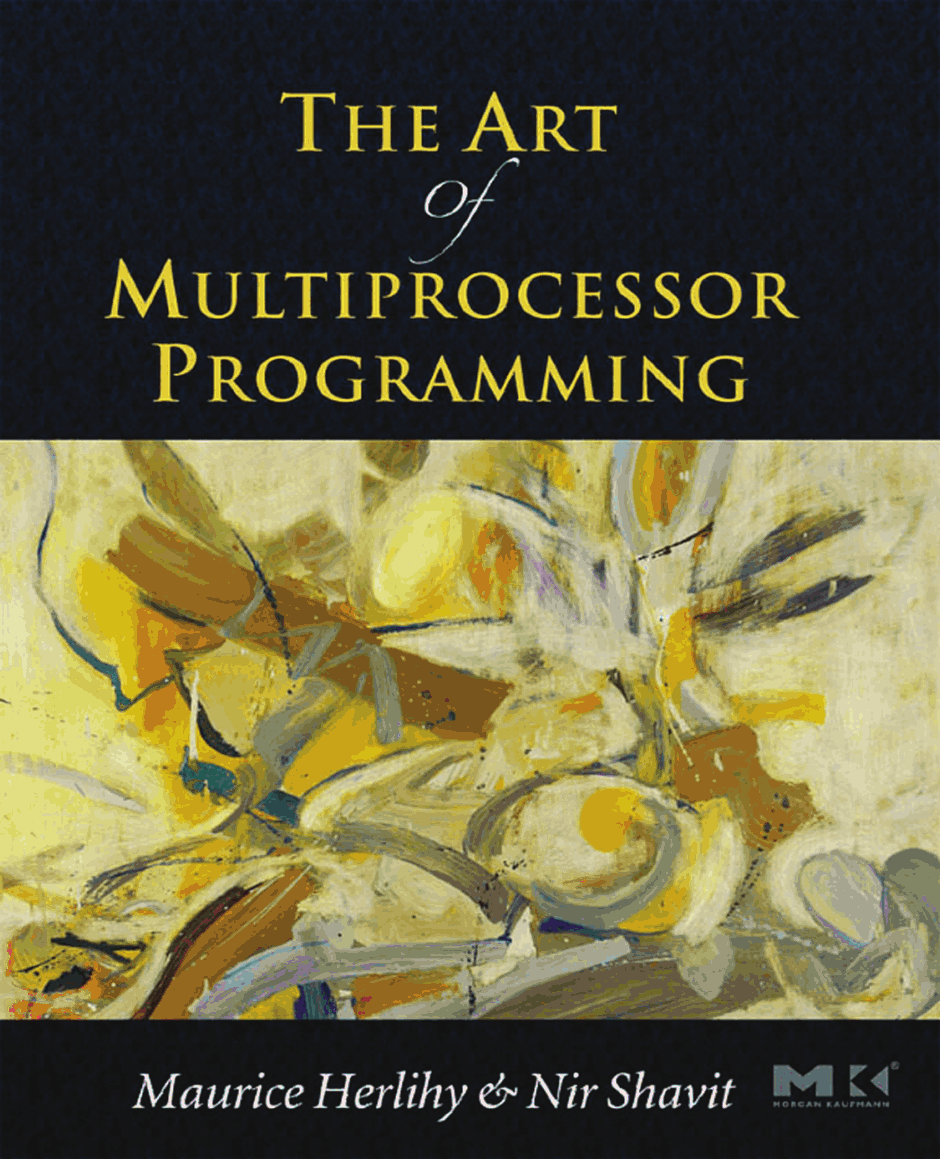
\includegraphics[scale=0.28]{figures/book-herlihy}
  \end{center}
\end{frame}

\begin{frame}{Thread Overhead}
  \begin{itemize}
  \item Threads require resources
    \begin{itemize}
    \item Memory for stacks
    \item Setup, teardown
    \end{itemize}
  \item Scheduler overhead
  \item Worse for short-lived threads
  \end{itemize}
\end{frame}

\begin{frame}{Thread Pools}
  \begin{itemize}
  \item More sensible to keep a pool of long-lived threads
  \item Threads assigned short-lived tasks
    \begin{itemize}
    \item Runs the task
    \item Rejoins pool
    \item Waits for next assignment
    \end{itemize}
  \end{itemize}
\end{frame}

\begin{frame}{Thread Pool = Abstraction}
  \begin{itemize}
  \item Insulate programmer from platform
    \begin{itemize}
    \item Big machine, big pool
    \item And vice-versa 
    \end{itemize}
  \item Portable code
    \begin{itemize}
    \item Runs well on any platform
    \item No need to mix algorithm/platform concerns
    \end{itemize}
  \end{itemize}
\end{frame}

\begin{frame}{\lstinline!ExecutorService! Interface}
  In \lstinline!java.util.concurrent!:

  \vspace{\stretch{1}}  

  \begin{itemize}
  \item Task = \lstinline!Runnable! object
    \begin{itemize}
    \item If no result value expected
    \item Calls \lstinline!run()! method.
    \end{itemize}
  \item Task = \lstinline!Callable<T>! object
    \begin{itemize}
    \item If result value of type \lstinline!T! expected
    \item Calls \lstinline!T call()! method.
    \end{itemize}
  \end{itemize}
\end{frame}

\begin{frame}[fragile]{\lstinline!Future<T>!}
\begin{lstlisting}
  Callable<T> task = ...; 
  ...
  Future<T> future = executor.submit(task);
  ...
  T value = future.get(); 
\end{lstlisting}

  \vspace{\stretch{1}}

  \begin{itemize}
  \item Submitting a \lstinline!Callable<T>! task returns a
    \lstinline!Future<T>! object
  \item The Future's \lstinline!get()! method blocks until the value
    is available
  \end{itemize}
\end{frame}

\begin{frame}[fragile]{\lstinline!Future<?>!}
\begin{lstlisting}
  Runnable task = ...; 
  ...
  Future<?> future = executor.submit(task);
  ...
  future.get(); 
\end{lstlisting}

  \vspace{\stretch{1}}

  \begin{itemize}
  \item Submitting a \lstinline!Runnable! task returns a
    \lstinline!Future<?>! object
  \item The Future's \lstinline!get()! method blocks until the
    computation is complete
  \end{itemize}
\end{frame}

\begin{frame}{Note}
  \begin{itemize}
  \item Executor Service submissions are purely advisory in nature
  \item The executor
    \begin{itemize}
    \item Is free to ignore any such advice
    \item And could execute tasks sequentially \ldots
    \end{itemize}
  \end{itemize}
\end{frame}

\begin{frame}{Fibonacci}
  \large{
    \begin{equation*}
      F(n) := 
      \begin{cases}
        1, & n = 0 \\
        1, & n = 1 \\
        F(n-1) + F(n-2), & n > 1
      \end{cases}
    \end{equation*}
  }

  \vspace{\stretch{1}}

  \begin{itemize}
  \item Potential parallelism
  \item Dependencies
  \end{itemize}
\end{frame}

\begin{frame}{Disclaimer}  
  \begin{itemize}
  \item This Fibonacci implementation is very inefficient
    \begin{itemize}
    \item So don’t deploy it!
    \end{itemize}
  \item But illustrates our point
    \begin{itemize}
    \item How to deal with dependencies  
    \end{itemize}
  \end{itemize}
\end{frame}

\begin{frame}[fragile]{Multithreaded Fibonacci}
\begin{lstlisting}[basicstyle=\fontsize{9}{11}\selectfont\ttfamily]
class FibTask implements Callable<Integer> {
  static ExecutorService exec = 
    Executors.newCachedThreadPool();
  int arg;
  public FibTask(int n) {
    arg = n;
  }
  public Integer call() {
    if (arg > 2) {
      Future<Integer> left = 
        exec.submit(new FibTask(arg-1));
      Future<Integer> right = 
        exec.submit(new FibTask(arg-2));
      return left.get() + right.get();
    } else {
      return 1;
    }
  }
}
\end{lstlisting}
\end{frame}


\section{New Assignment}

\begin{frame}{Outline}
  \tableofcontents[current]
\end{frame}

\begin{frame}{TODO}
  TODO
\end{frame}


\section*{Outro}

\begin{frame}{Summary}
  \begin{itemize}
  \item TODO
  \end{itemize}
\end{frame}

\end{document}
